Spotify là một nền tảng phát nhạc trực tuyến hàng đầu thế giới, cung cấp cho người dùng quyền truy cập vào hàng triệu bài hát, podcast và video từ các nghệ sĩ trên toàn cầu. Ra mắt vào năm 2008, Spotify đã thay đổi cách mọi người tiếp cận và thưởng thức âm nhạc, chuyển từ việc sở hữu bản ghi vật lý sang mô hình phát trực tuyến tiện lợi và hợp pháp.

Spotify hoạt động trên nhiều thiết bị, bao gồm máy tính, điện thoại di động, máy tính bảng, loa thông minh, TV và ô tô, cho phép người dùng nghe nhạc mọi lúc, mọi nơi. Nền tảng này cung cấp cả phiên bản miễn phí với quảng cáo và phiên bản trả phí (Spotify Premium) với nhiều tính năng nâng cao như nghe nhạc offline, chất lượng âm thanh cao hơn và không có quảng cáo. Spotify cũng nổi tiếng với khả năng cá nhân hóa trải nghiệm người dùng thông qua các playlist được tạo tự động dựa trên thói quen nghe nhạc, như "Discover Weekly" và "Daily Mix".

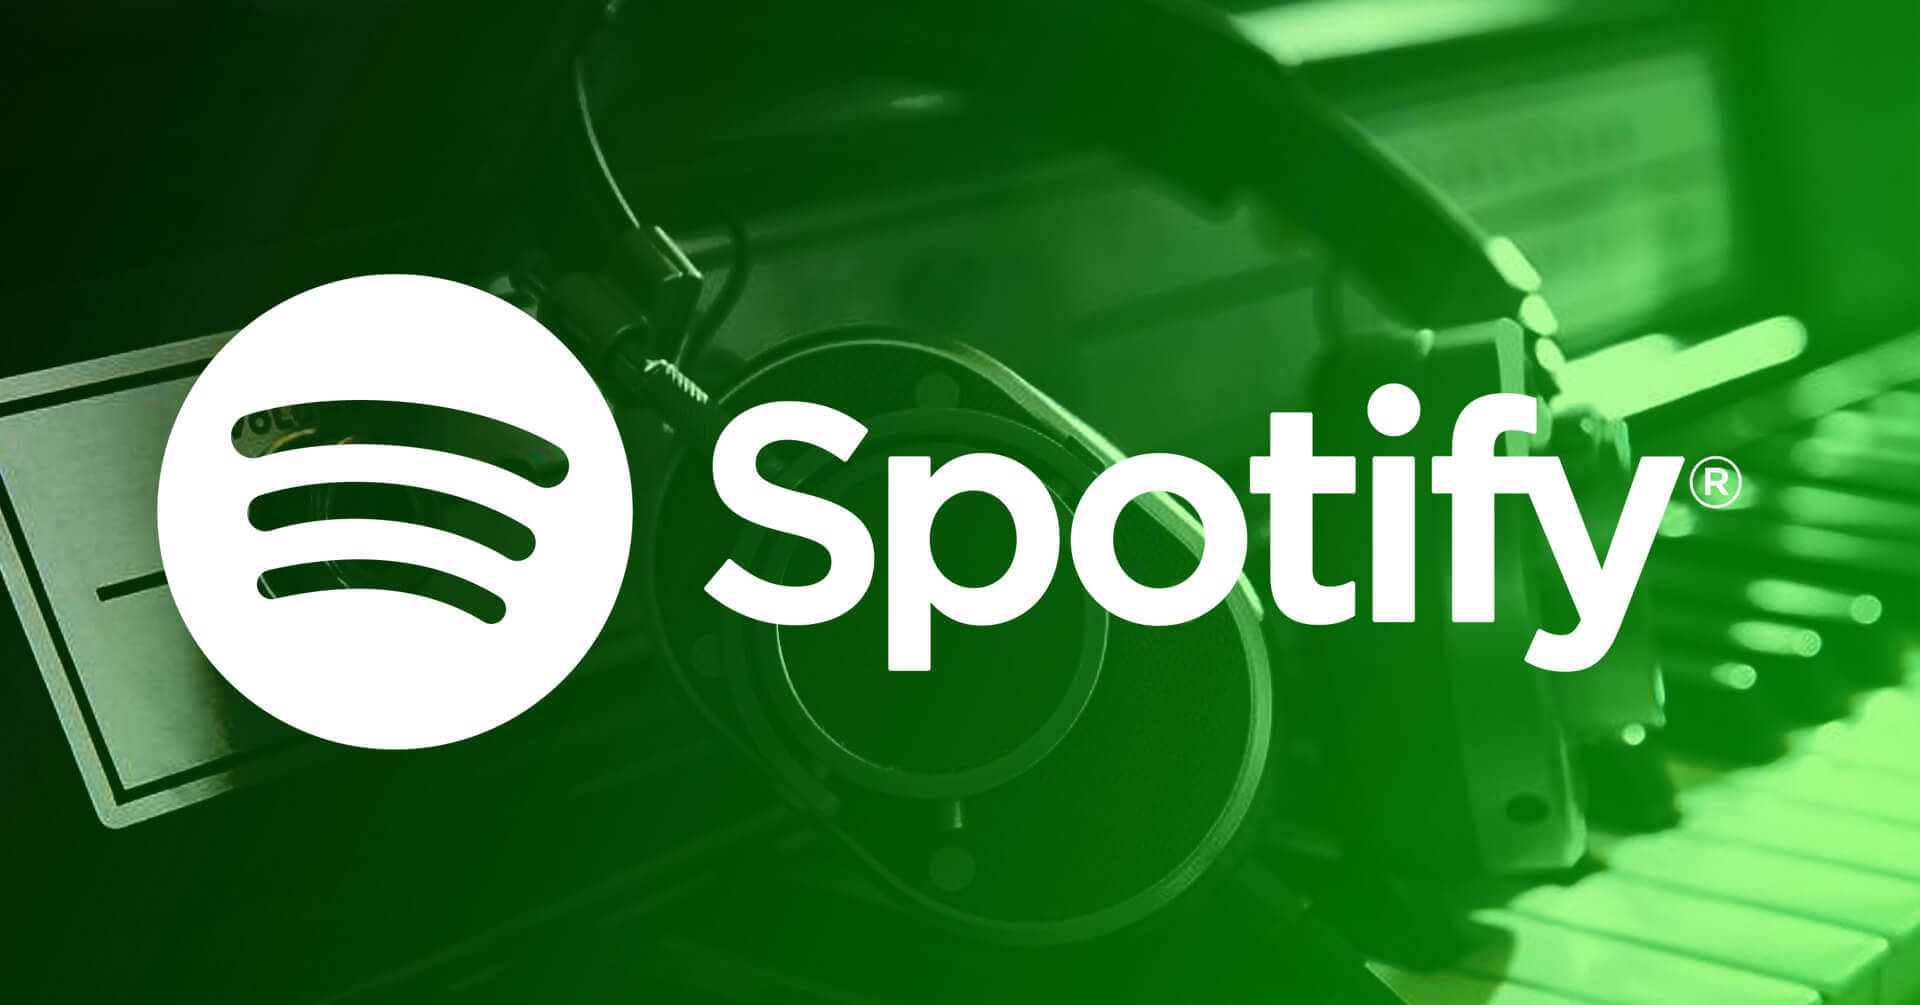
\includegraphics[width=\textwidth]{imgs/spotify.png}